\section{Hardware Design: Efficient Architecture}\label{sec:hardware}

In this section, we investigate the hardware level techniques used in state-of-the-art FPGA based neural network accelerator design to achieve high performance and high energy efficiency. We classify the techniques into 3 levels: computation unit level, loop unrolling level, and system level.

\subsection{Computation Unit Designs}\label{sec:hardware:cu}

Computation unit level design affect the peak performance of the neural network accelerator. With a certain FPGA chip, the available resource is limited. A smaller computation unit design means more computation units and higher peak performance. A carefully designed computation unit array can also increase the working frequency of the system and thus improve peak performance.

\subsubsection{Low Bit-width Unit}\label{sec:hardware:cu:lbu}
Reduce the number of bit-width for computation is a direct way to reduce the size of computation units. The feasibility of using less bits comes from the quantization methods as introduced in section~\ref{sec:software:quant}. Most of the state-of-the-art FPGA designs replace the 32-bit floating point units with fixed point units. Podili, et al.~\cite{podili2017fast} implements 32-bit fixed point untis for the proposed system. 16-bit fixed point units are widely adopted in \cite{qiu2016going, li2016high, xiao2017exploring, guan2017fp, zhang2016caffeine}. ESE~\cite{han2017ese} adopts 12-bit fixed-point weight and 16-bit fixed point neurons design. Guo, et al.~\cite{guo2017angel} use 8-bit units for their design on embedded FPGA. Recent work is also focusing on extremely narrow bit-width design. Prost-Boucle, et al.~\cite{prost2017scalable} implements 2-bit multiplication with 1 LUT for ternary network. Experiments in \cite{nurvitadhi2016accelerating} shows that FPGA implementation of Binarized Neural Network (BNN) outperforms that on CPU and GPU. Though BNN suffers from accuracy loss, many designs explore the benefit of using 1 bit for computation~\cite{li20177, nakahara2017batch, zhao2017accelerating, umuroglu2017finn, nakahara2017fully, jiao2017accelerating, moss2017high}.

The designs mentioned above are focused on computation unit for linear quantization. For non-linear quantization, translating the data back to full precision for computation is still of high cost. Samragh, et al.~\cite{samragh2017customizing} proposes the factorized coefficients based dot product implementation. As the possible values of weights are quite limited for non-linear quantization, the proposed computation unit accumulates the multiplicator for each possible value and calculate the result as the weighted sum of the values in look-up table. In this way, the multiplication needed for one output neuron is a constant as the number of values in look-up table. The original multiplications are replaced by random addressed accumulations.

Most of the designs use a same bit-width through the process of a neural network. Qiu, et al.~\cite{qiu2016going} finds that neurons and weights in FC layers can use less bits compared with CONV layers while the accuracy is maintained. Heterogeneous computation units are used in the designs of \cite{zhao2017accelerating, guo2017bit}.

The size of computation units of different bit-width is compared in Figure~\ref{fig:mac_util}. The resouce consumption is the synthesis result by Vivado 2017.2. All the IPs are required to not use DSP resources. Though we tend to use DSPs in real implementations, this result shows the actual hardware cost. It is also common to implement the computation units in a hybrid way like~\cite{qiu2016going}, where some of the operators are implemented by DSP and others by logic.

In neural network,the number of multiplication and addtion is approximately the same. So the sum of resource for multiplier and adder shows the overall cost. Operations with 32-bit fixed point data consumes similar resource as 32-bit floating point operations. For 16-bit operations, using fixed-point format saves about 30\% resource. As introduced in section~\ref{sec:software:quant}, 8-bit fixed point is the bound for linear quantization. Comapred with the 32-bit version, this allows 14$\times$ more hardware operators within the same area of logic. If further research can utilize 4-bit operations, this advantage becomes $54\times$.

\begin{figure}[t]
    \centering
    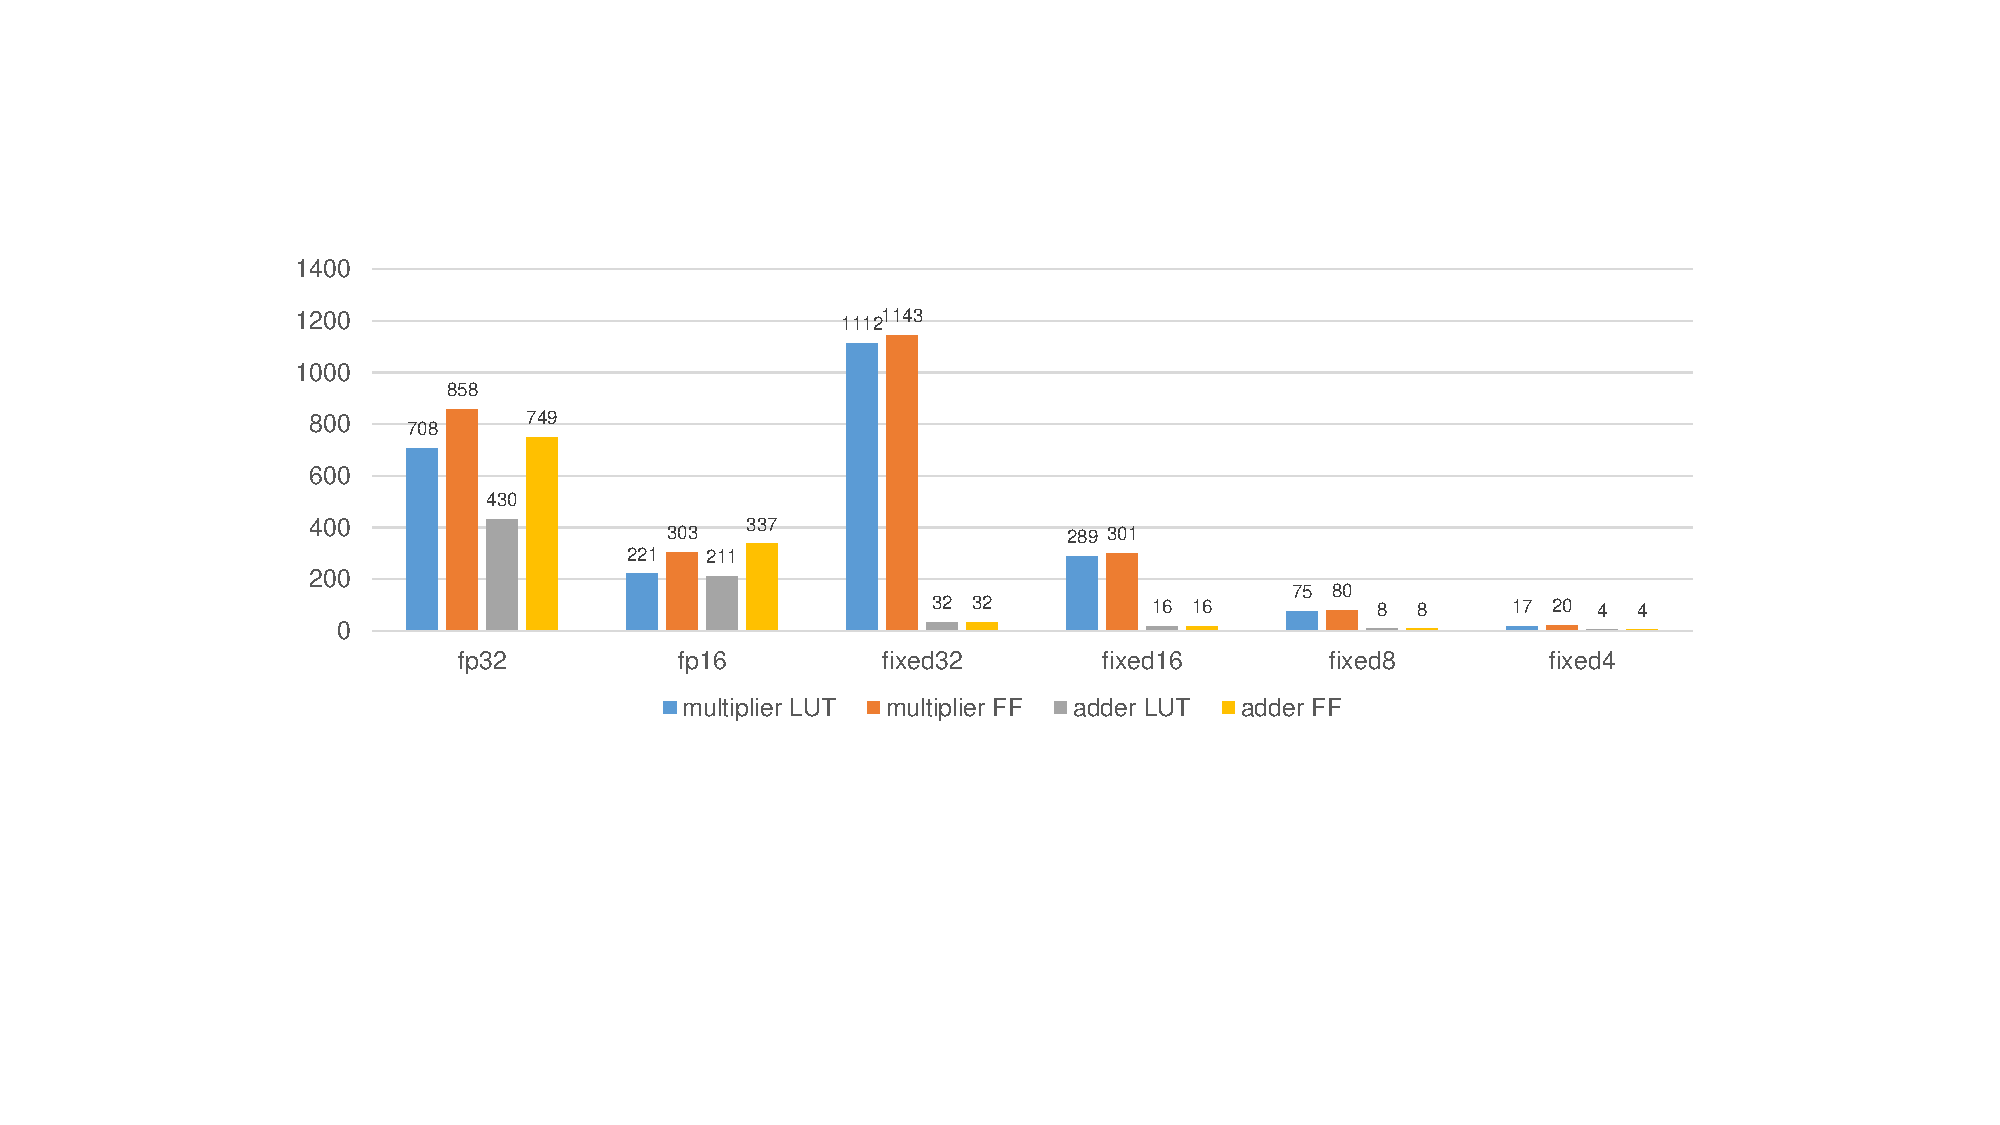
\includegraphics[width=1.0\columnwidth]{fig/mac_util.pdf}
    \caption{FPGA resource consumption comparison for multiplier and adder with different types of data.}
    \label{fig:mac_util}
\end{figure}

\subsubsection{Fast Convolution Unit}
For CONV layers, the convolution operations can be accelerated by special algorithms. Discrete Fourier Transformation (DFT) based fast convolution is widely adopted in digital signal processing. Zhang, et al.~\cite{zhang2017frequency} propose a 2D DFT based hardware design for efficient CONV layer execution. For an $F\times F$ filter convolved with $K\times K$ filter, DFT converts the $(F-K+1)^2K^2$ multiplications in sapce domain to $F^2$ complex multiplications in frequency domain. For a CONV layer with $M$ input channel and $N$ output channel, $MN$ times of frequency domain multiplications are needed while only $(M+N)$ times DFT/IDFT are needed. The conversion of convolution kernels is once for all. So the domain conversion process are of low cost for CONV layers. This technique does not work for CONV layers with stride>1 or $1\times 1$ convolution. Ding, et al.~\cite{ding2017c} suggests that a block-wise circular constraint can be applied on the weight matrix. In this way, the matrix vector multiplication in FC layers are converted to a set of 1D convolutions and can further accelerated in frequency domain. This method can also be applied to CONV layers by treating the $K\times K$ convolution kernels as $K\times K$ matrices and is not limited by $K$ or stride.

Frequency domain methods require complex number multiplication. Another kind of fast convolution involves only real number multiplication~\cite{winograd1980arithmetic}. The convolution of a 2D feature map $F_{in}$ with a kernel $K$ using Winograd algorithm is expressed by equation~\ref{eqt:winograd}.
\begin{equation}\label{eqt:winograd}
    F_{out} = A^T[(GF_{in}G^T)\odot(BF_{in}B^T)]A
\end{equation}
$G$, $B$ and $A$ are transformation matrix which only related to the sizes of kernel and feature map. $\odot$ denotes an element-wise multiplication of two matrices. For a $4\times 4$ feature map convolved with $3\times 3$ kernel, the transformation matrices are described as follows:
\begin{equation*}
    G = \left[
        \begin{array}{ccc}
            1           & 0            & 0           \\
            \frac{1}{2} & \frac{1}{2}  & \frac{1}{2} \\
            \frac{1}{2} & -\frac{1}{2} & \frac{1}{2} \\
            0           & 0            & 1
        \end{array}    
    \right] \quad
    B = \left[
        \begin{array}{cccc}
            1 & 0  & -1 & 0 \\
            0 & 1  & 1  & 0 \\
            0 & -1 & 1  & 0 \\
            0 & 1  & 0  & -1
        \end{array}
    \right] \quad
    A = \left[
        \begin{array}{cc}
            1 & 0  \\
            1 & 1  \\
            1 & -1 \\
            0 & -1 
        \end{array}
    \right]
\end{equation*}
Winograd based methods are also limited by the kernel size and stride as DFT based methods. The most commonly used Winograd transformation is for $3\times 3$ convolution in ~\cite{lu2017evaluating, xiao2017exploring}. 

\subsubsection{DSP Optimization}
Recent FPGAs implement hardened DSP units together with the reconfigurable logic to offer a high computation capacity. The basic function of a DSP unit is a multiplication accumulation (MAC). The bit-width for multiplication and addition is fixed. When the bit-width used in neural network does not match that of the DSP units, the FPGA is not fully utilized. The latest DSP units in Altera's FPGA implements 2 $18\times 19$ multipliers and can be configured into a $27\times 27$ multiplier or a 32-bit floating point multiplier~\cite{altera_dsp}. That of Xilinx's FPGA implements one $27\times 18$ multiplier~\cite{xilinx_dsp}. As mentioned in section~\ref{sec:hardware:cu:lbu}, many designs adopt multiplication with less or equal than 16 bits, which can cause great DSP under utilization.

Nguyen, et al.~\cite{nguyen2017double} propose the design to implement two narrow bit-width fixed-point multiplication with a single wide bit-width fixed-point multiplier. In this design, $AB$ and $AC$ is executed with one multiplication $A(B<<k+C)$. If $k$ is sufficiently large, the bits for $AB$ and $AC$ does not overlap in the multiplication result and can be directly seperated. The design in~\cite{nguyen2017double} implements two 8-bit multiplications with one $25\times 18$ multiplier, where $k$ is 9. Similar method can be applied on other bit-width and DSPs.

\subsubsection{Frequency Optimization Methods}
All the above techniques introduced targets at increasing the number of computation units within a certain FPGA. Increasing the working frequency of the computation units also improves the peak performance.

To implement high parallelism, neural network accelerators usually implements matrix-vector multiplication or matrix-matrix multiplications rather than vector inner product as the basic operation. Different computation units share operators. Simply broadcast data to different computation units leads to large fan-out and high routing cost and thus reduce the working frequency. Wei, et al.~\cite{wei2017automated} use the systolic array structure in their design. The shared data are transferred from one computation unit to the next in a chain mode. So the data is not broadcasted and only local connections between different computation units are needed. The drawback is the increase in latency. As the process of a neural network model is determined and the systolic structure is fully pipelined, the latency overhead can be fully covered.

Latest FPGAs support 700-900MHz DSP theoretical peak working frequency. But existing designs usually work at 100-300MHz~\cite{qiu2016going, guo2017angel, zhang2016caffeine, ma2017optimizing}. As claimed in \cite{wu2017high}, the working frequency is limited by the routing between on-chip SRAM and DSP units. The design in \cite{wu2017high} use different working frequencies for DSP units and surrounding logic. Neighbour slices to each DSP unit are used as local RAMs to separate the clock domain. The prototype design in \cite{wu2017high} achieves the peak DSP working frequency at 741MHz and 891MHz on FPGA chips of different speed grades. Yet this method is not adopted by a complete neural network accelerator design. 

\subsection{Loop Unrolling Strategies}\label{sec:hardware:lu}
CONV layers and FC layers contribute to most of the computations and storage requirment of a neural network. As introduced in section~\ref{sec:preliminary}. We express the CONV layer function in equation~\ref{eqt:conv} as nested loops in Algorithm~\ref{alg:conv}. To make the code clear to read, we merge the loops along $x$ and $y$ directions for feature maps and 2-D convolution kernels respectively. An FC layer can be treated as a CONV layer with feature map and kernel both of size $1\times 1$. Besides the loops in Algorithm~\ref{alg:conv}, we also parallelize the process of multiple inputs as a batch. This forms the batch loop.

\begin{algorithm}  
    \caption{Convolution Layer}
    \label{alg:conv}
    \begin{algorithmic}[1]
        \Require feature map $F_{in}$ of size $M\times Y\times X$; 
                 convolution kernel $Ker$ of size $N\times M\times K\times K$;
                 bias vector $b$ of size $N$ 
        \Ensure  feature map $F_{out}$
        \Function {ConvLayer}{$F_{in}, Ker$}  
            \State Let $F_{out} \gets $ zero array of size $N\times(Y-K+1)\times(X-K+1)$  
            \For{$n=1$; $n<N$; $n++$} \Comment Output channel loop
                \For{$m=1$; $m<M$; $m++$} \Comment Input channel loop
                    \For{each $(y, x)$ within $(Y-K+1, X-K+1)$} \Comment Feature map loop
                        \For{each $(ky, kx)$ within $(K, K)$} \Comment Kernel loop
                            \State $F_{out}[n][y][x] += F_{in}[m][y-ky+1][x-kx+1] * K[n][m][ky][kx]$
                        \EndFor
                    \EndFor
                \EndFor
                \State $F_{out}[n] += b[n]$
            \EndFor
            \State \Return{$F_{out}$}
        \EndFunction  
        
    \end{algorithmic}  
\end{algorithm}

To parallelize the execution of the loops, we unroll a certain part of the loops and map every operation in this part as a hardware computation unit. An imappropriate set of loop unroll parameter may lead to serious hardware underutilization. We take an example of three nested loops as shown in Figure~\ref{fig:unrolling}. The big cube denotes all the operations within the loops. The length of each edge denotes the trip count of a loop. The small cube denotes the unrolled kernel, whose edges denote the unrolling parameter. A complete execution of the workload means to fullfill the big cube with small cubes. Figure~\ref{fig:unrolling}(a) shows an appropriate set of unroll parameters. But for Figure~\ref{fig:unrolling}(b), the red part of some of the small cubes are out of the big cube, which means the hardware is wasted.

\begin{figure}[t]
    \centering
    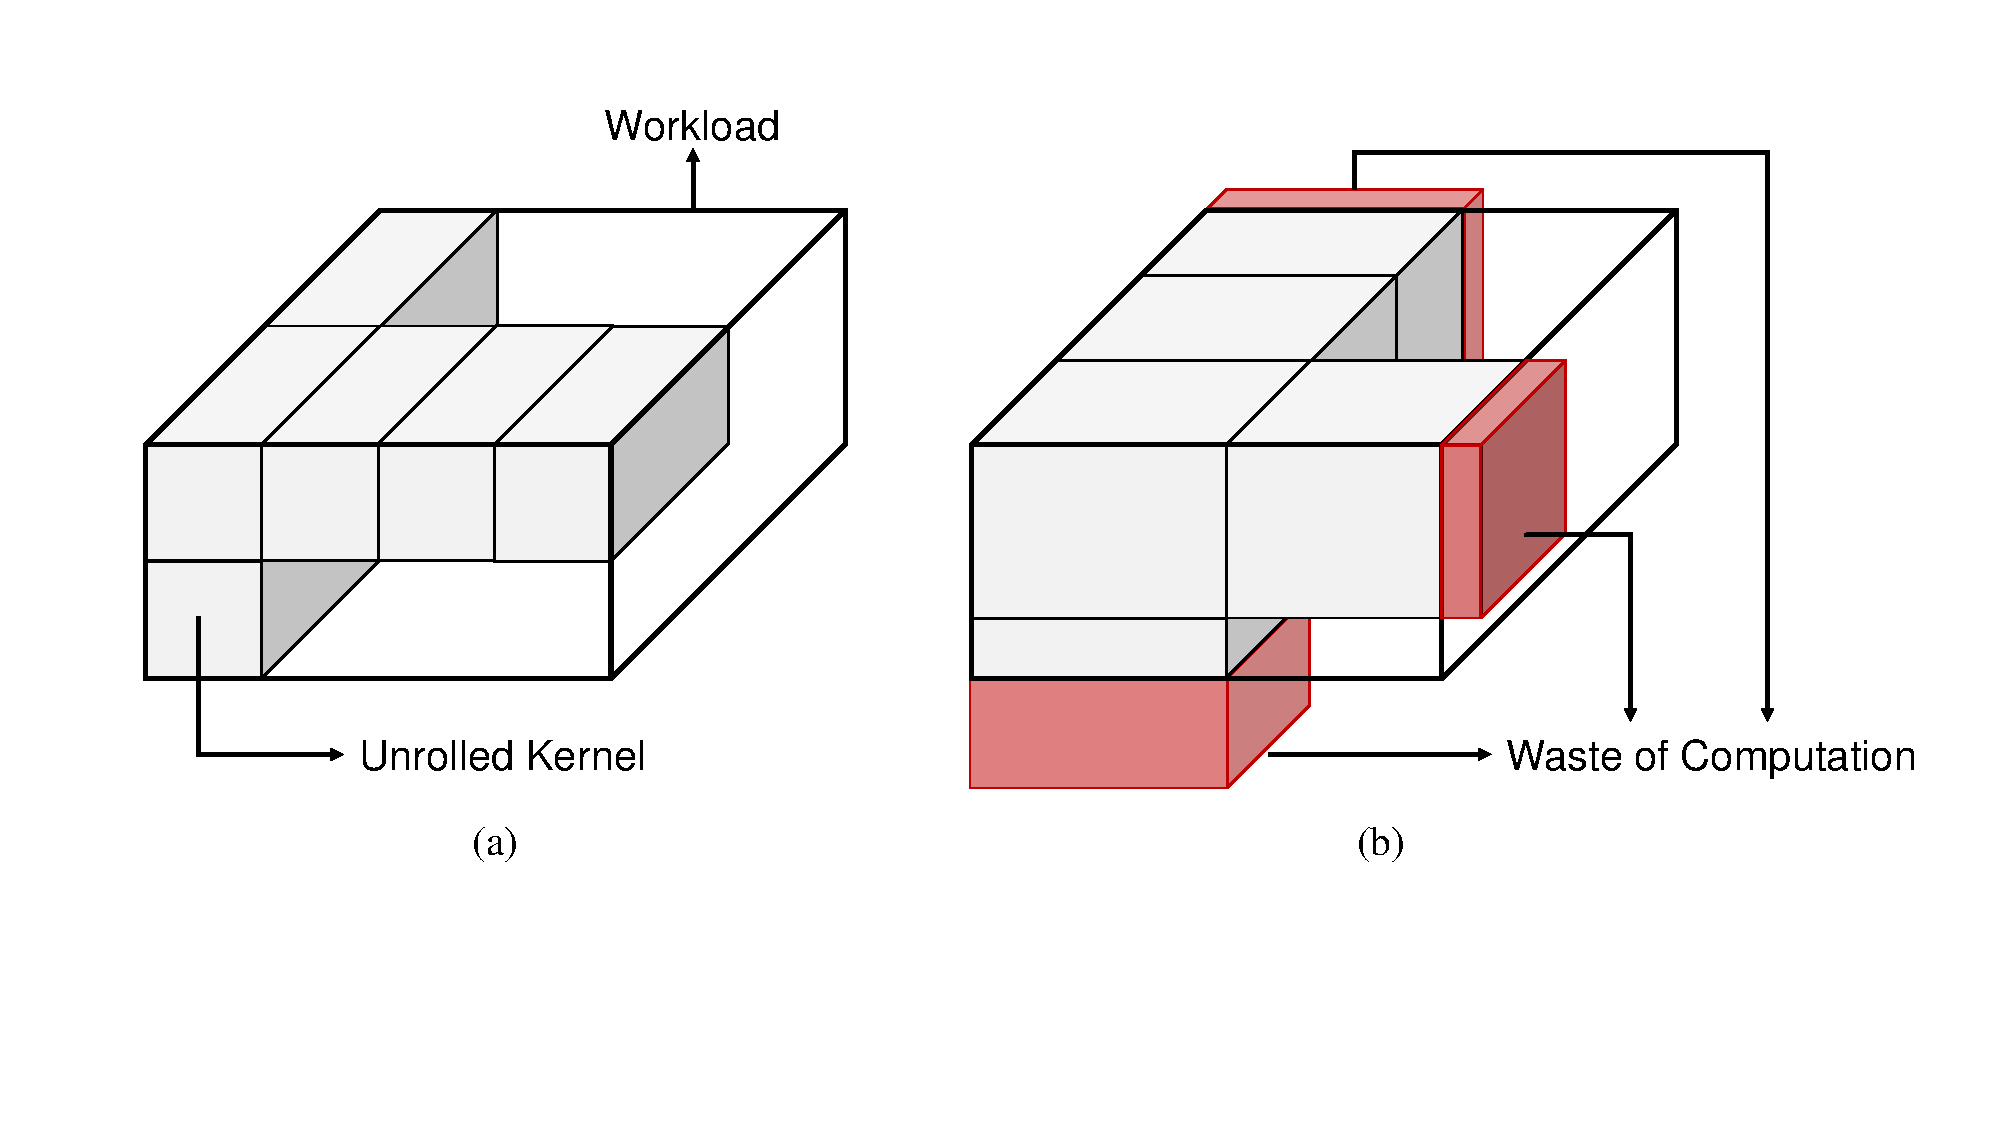
\includegraphics[width=0.8\columnwidth]{fig/unrolling.pdf}
    \caption{Comparison between appropriate and inappropriate loop unroll parameters. (a) Appropriate parameters. (b) Inappropriate parameters.}
    \label{fig:unrolling}
\end{figure}

It is obvious from Figure~\ref{fig:unrolling} that if the trip count of a loop is too small, the unroll parameter for this loop is limited. For a CNN model, the loop dimension varies greatly among different layeres. For a common network used on ImageNet classification like ResNet~\cite{he2016deep}, the channel numbers vary from 3 to 2048, the feature map sizes vary from $224\times 224$ to $7\times 7$, the convolution kernel sizes vary from $7\times 7$ to $1\times 1$. Besides the under utilization problem, loop unrolling also affect the datapath and on-chip memory design. Thus loop unrolling strategy is a key feature for a neural network accelerator design. 

Various work are proposed focusing on how the unroll parameter should be chosen. Zhang, et al.~\cite{zhang2015optimizing} propose the idea of unrolling the input channel and output channel loops and choose the optimized unroll parameter by design space exploration. Along these two loops, there is no input data cross dependency between neighbouring iterations. So no multiplexer is needed to rounte data from on-chip buffer to computation units. But the parallelism is limited as $7\times 64=448$ multipliers. For larger parallelism, this solution is easy to suffer from the under utilization problem. Ma, et al.~\cite{ma2017optimizing} further extends the design space by allowing parallelism on the feature map loop. The parallelism reaches $1\times 16\times 14\times 14=3136$ multipliers. A shift register structure is used to route feature map pixels to the computation units.

The kernel loop is not chosen in the above work because kernel sizes vary greatly. Motamedi, et al~\cite{motamedi2016design} analysis the kernel unrolling on AlexNet. Even with $3\times 3$ unroll for the $11\times 11$ and $5\times 5$ kenrels, the overall system performance still reaches 97.4\% of its peak performance for the convolution layers. For certain networks like VGG~\cite{simonyan2014very}, only $3\times 3$ convolution kernels are used.  Qiu, et al.~\cite{qiu2016going} use the line-buffer structure to achieve $3\times 3$ sliding window function and fully parallelize the kernel loop. Another reason to unroll kernel loop is to achieve acceleration with fast convolution algorithms. Design in \cite{zhang2017frequency} implements fully parallelized frequency domain multiplication on $4\times 4$ feature map and $3\times 3$ kernel. Lu, et al.~\cite{lu2017evaluating} implement Winograd algorithm on FPGA with a dedicated pipeline for equation~\ref{eqt:winograd}. The convolution of $3\times 3$ kernel on $6\times 6$ kernel is fully paralleized.

The above solutions are only for a single layer. But there is hardly a one-size-fits-all solution for a whole network, especially when we need high parallelism. Designs in \cite{li2016high, liu2016automatic} propose fully pipelined structure with each layer a pipe stage. As each layer is executed with an independent part of hardware and each part is small, loop unrolling method can be easily chosen. But this method is memory consuming because ping-pong buffers are needed between neighbouring layers for the feature maps. Design in \cite{zhang2016energy} is similar but implemented on FPGA clusters to resolve the scalability problem. Shen, et al.~\cite{shen2016overcoming} group the layers of a CNN by the loops' trip count and map each group onto one hardware module. Actuallly these solutions can be treated as unrolling the batch loop, because different inputs are processed in parallel on different layer pipe stage. The design in \cite{lu2017evaluating} implements parallelized batch both within a layer and among different layers. The drawback of batch parallel method is that the latency is higher compared with a $batch=1$ design of a same parallelism.

Most of the current designs follow one of the above methods for loop unrolling. A special kind of design is for sparse neural network. Han, et al.~\cite{han2017ese} propose the ESE architecture for sparse LSTM network acceleration. Unlike processing a dense network, all the computation units will not work synchronously. This causes difficulty in sharing data between different computation units. ESE implements only the output channel (the output neurons of the FC layers in LSTM) loop unroll within a layer to simplify hardware design and parallelize batch process.

\subsection{System Design}

A typical FPGA based neural network accelerator system is shown in Figure~\ref{fig:sys}. The logic part of the whole system are denoted with the blue boxes. The host CPU issues workload or commands to the FPGA logic part and monitors its working status. On the FPGA logic part, a controller is usually implemented to communicate with host and generates control signals to all the other modules on FPGA. The controller can be an FSM or an instrcution decoder. The on the fly logic part is implemented for certain designs if the data loaded from external memory needs preprocess. This module can be data arrangement module, data shifter~\cite{qiu2016going}, FFT module~\cite{zhang2017frequency}, etc. The computation units are as discussed in section~\ref{sec:hardware:cu} and section~\ref{sec:hardware:lu}.

\begin{figure}[t]
    \centering
    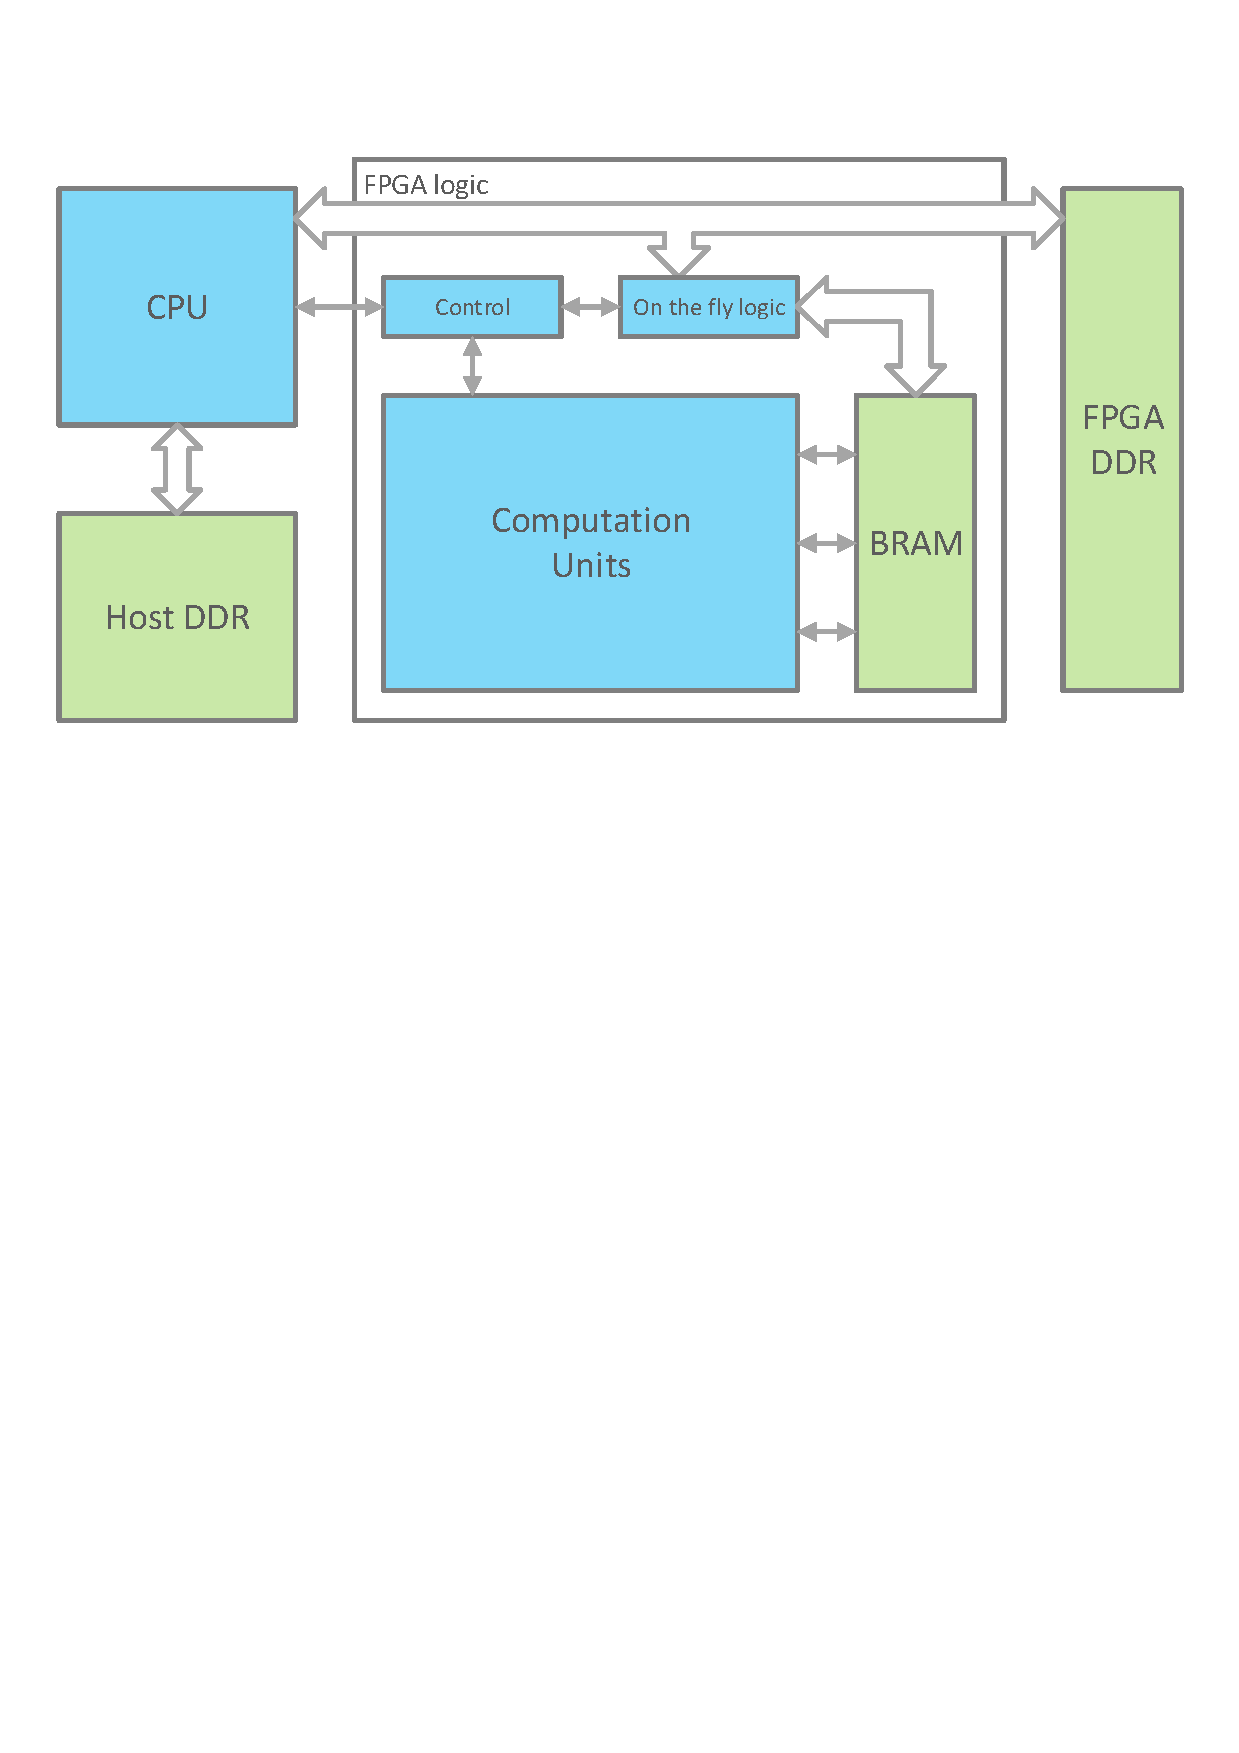
\includegraphics[width=0.8\columnwidth]{fig/sys.pdf}
    \caption{Block graph of a typical FPGA based neural network accelerator system}
    \label{fig:sys}
\end{figure}

The memory hiearchy of the system mainly contains three parts, denoted as the green boxes in Figure~\ref{fig:sys}: Host DDR, FPGA DDR and on-chip block RAM. For state-of-the-art network, 
